Blood Bowl to strategiczna gra planszowa łącząca elementy footballu amerykańskiego oraz gier bitewnych. Rozgrywka toczy się na planszy w formie boiska o wymiarach 26×15 pól. Dwóch graczy prowadzi przeciwne drużyny złożone z figurek (zwanych zawodnikami) i dąży do zdobycia większej liczby przyłożeń (ang. touchdown) niż przeciwnik. Mecz składa się z dwóch połówek po 8 tur dla każdego gracza. W każdej turze trener może aktywować wielu swoich zawodników, wykonując nimi szereg akcji na boisku. Do podstawowych typów akcji należą m.in.: ruch (przesunięcie zawodnika o kilka pól zależnie od jego parametru szybkości), podanie piłki, przekazanie piłki innemu zawodnikowi (ang. handoff), blok (atak na sąsiadującego przeciwnika w próbie powalenia go), blitz (połączenie ruchu i ataku), a nawet sfaulowanie leżącego przeciwnika (ang. foul). Gdy zawodnik z piłką dotrze do strefy punktowej rywala, jego drużyna zdobywa punkt. Po upływie ustalonej liczby tur mecz kończy się, a wygrywa drużyna z większą liczbą przyłożeń.

Istotnym elementem Blood Bowl jest losowość oraz wynikające z niej zarządzanie ryzykiem. Większość istotnych akcji – takich jak bloki, uniki, podania czy chwyt piłki – wymaga powodzenia testu kośćmi. Szanse zależą od atrybutów zawodników (np. Siły przy blokowaniu, Zręczności przy chwytaniu czy uniku) oraz posiadanych umiejętności specjalnych (np. Dodge, Block). Niepowodzenie testu zwykle oznacza natychmiastową utratę tury (tzw. turnover). W związku z tym trenerzy muszą rozważnie planować kolejność działań – zazwyczaj zaczynają od ruchów bezpiecznych (niewymagających rzutów lub z bardzo dużą szansą powodzenia), odkładając ryzykowne akcje na koniec tury. Gra przyznaje też ograniczoną liczbę żetonów przerzutów, które pozwalają powtórzyć nieudany rzut kością, co dodaje element decyzyjny dotyczący zarządzania zasobami szczęścia. Stan gry w Blood Bowl jest złożony i bogaty: obejmuje on nie tylko położenie wszystkich zawodników na planszy, ale również ich stan (stojący, powalony, ogłuszony itp.), posiadane atrybuty i umiejętności, stan piłki, warunki pogodowe, licznik tur, rezerwy i kontuzje graczy w drużynach, dostępne przerzuty i inne elementy. W odróżnieniu od gier takich jak Go czy szachy, reprezentacja stanu w Blood Bowl ma charakter wielowymiarowy przestrzennie oraz nieprzestrzennie, a przestrzeń akcji nie jest stała – dostępne ruchy zależą od kontekstu sytuacyjnego każdego kroku.
 
\vspace{6mm}
\begin{figure}[!hb]
	\centering 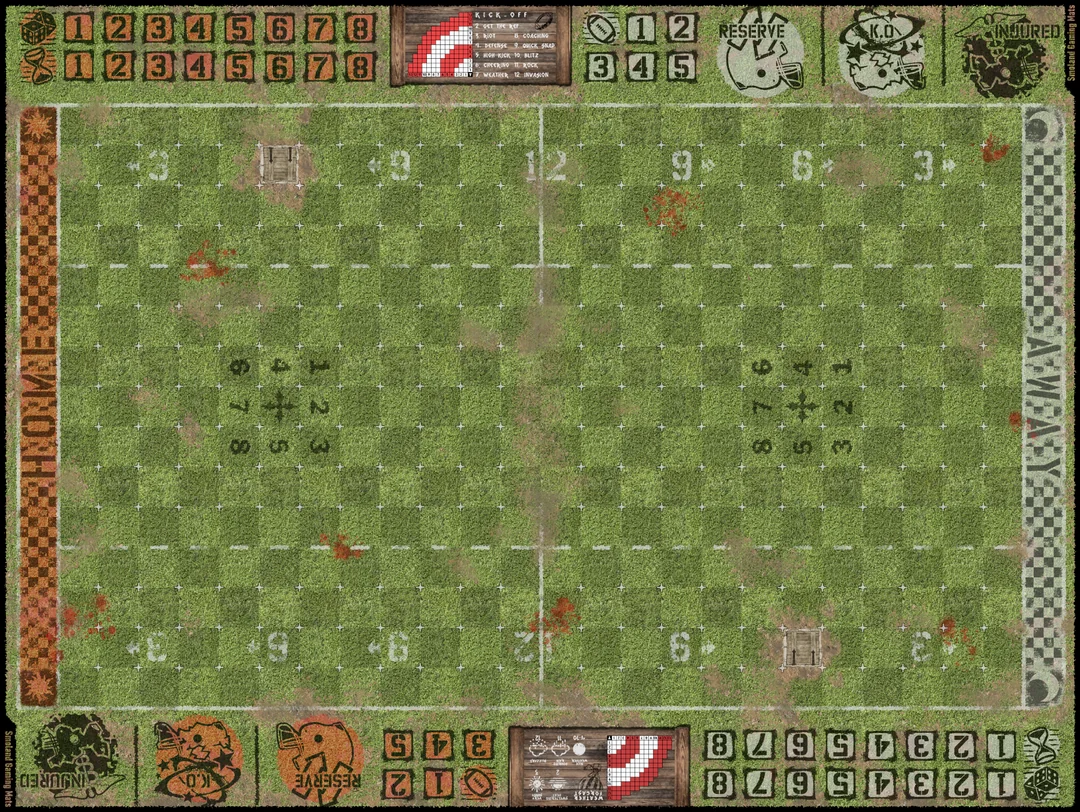
\includegraphics[width=\textwidth]{rysunki/Botbowl_board.jpg} % rysunek o szerokości 0.618 długości linii tekstu - złoty podział
	\caption{Plansza Blood Bowl}
	\label{Plansza Bloodbowl}
\end{figure}


\section{Blood Bowl jako benchmark dla uczenia ze wzmocnieniem.}

Blood Bowl jest uważany za kolejne wielkie wyzwanie dla sztucznej inteligencji w grach planszowych
njustesen.github.io
. Kilka cech tej gry sprawia, że stanowi ona wartościowe środowisko testowe dla metod uczenia ze wzmocnieniem i sieci neuronowych:
\begin{enumerate}
	\item Wysoki branching factor – Każda tura oferuje olbrzymią liczbę możliwych sekwencji ruchów. Trener może poruszać wieloma zawodnikami w dowolnej kolejności, a każdy z nich może wykonać kilka akcji. Średni współczynnik rozgałęzienia pojedynczej akcji zawodnika szacuje się na ok. $10^5$ możliwych przebiegów. W rezultacie pojedyncza tura (maksymalnie ~10 zawodników) może rozwidlać się nawet na rząd $~10^{50}$ możliwych ciągów akcji. Dla porównania, w szachach średni współczynnik rozgałęzienia wynosi ok. 30, a w go ok. 300. Tak ogromna przestrzeń decyzji przekracza możliwości tradycyjnych algorytmów przeszukiwania i stanowi poważne wyzwanie dla metod RL.
	\item Nieregularne drzewa decyzyjne – W Blood Bowl długość tury oraz dostępne akcje nie są z góry ustalone. Z jednej strony, lista dozwolonych ruchów w danym momencie zależy od stanu gry (np. tylko niektórzy zawodnicy mogą wykonać określone akcje, możliwe pola ruchu są ograniczone zasięgiem, itp.), co oznacza dynamicznie zmieniającą się przestrzeń akcji. Z drugiej strony, wskutek losowości tura gracza może zakończyć się wcześniej (np. nieudany rzut kończy turę), przez co drzewo rozgrywki ma zmienną głębokość gałęzi. Strukturę decyzyjną Blood Bowl można określić jako niestandardową lub zagnieżdżoną: tura składa się z serii ruchów zawodników (podtur), z których każdy z kolei bywa sekwencją kilku akcji (np. ruch przez kilka pól, a następnie blok). Taka nieregularność utrudnia zastosowanie klasycznych algorytmów planowania, które zakładają stałą liczbę ruchów na turę i jednolitą strukturę drzewa.
	\item Wieloetapowy charakter rozgrywki – Blood Bowl wymaga długoterminowego planowania oraz podejmowania szeregu skorelowanych decyzji w ramach jednej tury i całego meczu. Pełna rozgrywka to kilkanaście tur na stronę, łącznie około 1600 kroków decyzyjnych według szacunków. Punkty (przyłożenia) są zdobywane rzadko – w wielu partiach pada bardzo mało goli, zwłaszcza przy losowej lub słabej grze zdarza się remis 0:0. Taka długa horyzontalnie sekwencja decyzji ze sporadyczną nagrodą (sparse reward) powoduje, że algorytmy oparte na przeszukiwaniu oraz klasyczne metody RL mają trudność z uzyskaniem sygnału uczącego. Konieczne jest więc planowanie wieloetapowe – zarówno taktyczne (w obrębie jednej tury, optymalna kolejność akcji pod ryzykiem turnover), jak i strategiczne (przez cały mecz, np. zabezpieczenie piłki, kontrola czasu gry itp.).
	\item  Aspekty przestrzenne gry – Gra ma wyraźny charakter przestrzenny: położenie zawodników na planszy i kontrola terytorium (strefy ataku, krycie przeciwników, droga do pola punktowego) są kluczowe dla sukcesu. Stan gry można przedstawić w formie siatki cech (mapy zajętości pól, stref wpływu, pozycji piłki, itp.), co przypomina reprezentacje stanów znane z gier takich jak StarCraft II. Równocześnie jednak Blood Bowl posiada elementy symboliczne i atrybutowe (cechy postaci, liczniki, efekty), których nie da się ująć wyłącznie na obrazowej planszy. Ta kombinacja informacji przestrzennej i nieprzestrzennej wymaga od agentów uczenia się zarówno rozumienia układów geometrycznych na polu gry, jak i śledzenia zmiennych nienumerycznych (punkty, przerzuty, statusy). Stanowi to dobre pole do badań nad połączeniem sieci konwolucyjnych służących do przetwarzania map cech z sieciami gęstymi lub mechanizmami uwagi, analogicznie do podejść stosowanych w środowisku StarCraft II Learning Environment (SC2LE) \cite{Vinyals2017SC2LE}.
\end{enumerate}

\section{Środowisko BotBowl}
W celu badania opisanych wyżej zagadnień, stworzono BotBowl – otwartoźródłowe środowisko symulujące pełne zasady Blood Bowl, znane też jako Fantasy Football AI (FFAI). Platforma ta dostarcza szereg funkcjonalności wspierających efektywne szkolenie agentów sztucznej inteligencji.

BotBowl udostępnia interfejs zgodny z popularnym schematem OpenAI Gym, co ułatwia integrację z istniejącymi algorytmami RL. Środowisko zostało zaimplementowane w języku Python, dzięki czemu można bezpośrednio korzystać z bibliotek uczenia maszynowego, a sam interfejs obejmuje standardowe metody jak reset() (inicjalizacja nowej gry) oraz step(akcja) (wykonanie kroku).

Framework BotBowl umożliwia łatwe tworzenie i włączenie własnych agentów. Udostępniane jest API wysokiego poziomu: wystarczy zaimplementować klasę bota dziedziczącą po abstrakcyjnej klasie Agent (z metodami m.in. act() definiującą decyzje na podstawie stanu gry). Następnie takiego bota można zarejestrować w systemie pod unikalną nazwą i używać go w symulacjach lub turniejach. BotBowl zawiera też przykładowe zaimplementowane boty (np. losowy RandomBot, heurystyczny GrodBot) mogące służyć jako punkt wyjścia lub przeciwnicy do testów.

Środowisko pozwala na resetowanie stanu gry oraz rozgrywanie meczów między wybranymi agentami w trybie symulowanym bez interakcji użytkownika. Możliwe jest również równoległe uruchamianie wielu instancji gry (multi-env) w celu przyspieszenia treningu. Dodatkowo BotBowl zawiera forward model (silnik przewidywania następstw akcji), co umożliwia zastosowanie metod planowania czy przeszukiwania drzewa gry (np. MCTS (ang. \textit{Monte Carlo tree search})) obok czystego RL. Wbudowane funkcje turniejowe pozwalają automatycznie rozegrać serię gier między botami, kontrolując limity czasu na turę oraz wykrywając ewentualne zawieszenia lub awarie agentów (co jest istotne przy treningu i testowaniu na szeroką skalę).

Stan rozgrywki zwracany przez środowisko jest podzielony na część przestrzenną i nieprzestrzenną. Część przestrzenna to tensor wymiaru $(L, H, W)$, gdzie $H \times W$ odpowiada polu gry (wraz z ewentualnymi obrzeżami), zaś $L$ to liczba warstw cech. Domyślnie dostarczanych jest kilkadziesiąt warstw, m.in. zajętość pola przez zawodników, strefy ataku, pozycja piłki, pola dostępne do ruchu, prawdopodobieństwa powodzenia rzutów itp. . Część nieprzestrzenna to wektor liczbowy zawierający inne informacje o stanie gry – np. liczba tur, punkty, pozostałe przerzuty obu drużyn, aktualna faza/procedura gry – a także wskazania, które typy akcji są obecnie dostępne. Co ważne, BotBowl dostarcza również maskę dozwolonych akcji, dzięki czemu agent otrzymuje informację, które konkretne akcje (z ogromnej puli wszystkich możliwych) są w danym momencie legalne. Przestrzeń wszystkich potencjalnych akcji jest bowiem bardzo duża – rzędu tysięcy możliwych kodowanych decyzji – jednak w danej sytuacji tylko niewielki podzbiór ruchów wchodzi w grę. Maska (oraz alternatywnie struktura danych game.state.available\_actions) pozwala ograniczyć wybór do ruchów legalnych, co znacznie ułatwia trenowanie modelu i konwergencję algorytmów RL.

Podsumowując, Blood Bowl dostarcza unikalne, wymagające środowisko o wysokiej złożoności, które dzięki platformie BotBowl jest dostępne do eksperymentów z algorytmami uczenia ze wzmocnieniem. Połączenie czynników takich jak ogromny współczynnik rozgałęzienia, losowość i wieloetapowość decyzji oraz potrzeba percepcji przestrzennej czyni z niego atrakcyjny poligon doświadczalny dla nowoczesnych metod AI. BotBowl zapewnia zaś odpowiednie narzędzia – od interfejsu Gym, poprzez bogatą reprezentację stanów i mechanizmy ułatwiające implementację własnych agentów, aż po możliwość symulacji gier na masową skalę – aby skutecznie trenować i testować modele uczące się gry w Blood Bowl \cite{botbowl_docs}.

\section{Przegląd najlepszych rozwiązań w środowisku BotBowl}

Poniżej przedstawiono zestawienie rozwiązań osiągających najlepsze wyniki w kolejnych edycjach konkursu BotBowl. Wyróżniono osobno zwycięzców całych edycji konkursu oraz najwyżej sklasyfikowane rozwiązania wykorzystujące uczenie maszynowe, ponieważ w BotBowl najlepsze wyniki ogólne nie zawsze były uzyskiwane przez modele uczone.

\begin{table}[H]
	\centering
	\caption{Zwycięskie modele BotBowl}
	\label{tab:botbowl-sota}
	\begin{tabular}{lll}
		\hline
		Edycja & Bot & Podejście \\
		\hline
		Bot Bowl I & GrodBot & reguły eksperckie \\
		Bot Bowl II & Minigrod & reguły eksperckie  \\
		Bot Bowl III & MimicBot & imitation learning + RL \\
		Bot Bowl IV & Drefsante AI & bot ekspercki / heurystyczny  \\
		Bot Bowl V & Drefsante AI & bot ekspercki / heurystyczny  \\
		\hline
	\end{tabular}
\end{table}

\begin{table}[H]
	\centering
	\caption{Najlepsze rozwiązania wykorzystujące uczenie maszynowe w kolejnych edycjach BotBowl}
	\label{tab:botbowl-sota-ml}
	\begin{tabular}{llll}
		\hline
		Edycja & Bot & Podejście & Wynik / rola \\
		\hline
		Bot Bowl I & NO ONE & A2C, self-play, reward shaping & 3. miejsce \\
		Bot Bowl II & Gotebot & A2C, self-play, curriculum learning & 4. miejsce\\
		Bot Bowl III & MimicBot & imitation learning + RL & 1. miejsce, nagroda ML \\
		Bot Bowl IV & MotBot & uczenie maszynowe & 2. miejsce \\
		Bot Bowl V & Treeman & uczenie maszynowe / techniki ML lub search & 3. miejsce \\
		\hline
	\end{tabular}
\end{table}


Na podstawie tabeli \ref{tab:botbowl-sota} można zauważyć, że w kolejnych edycjach konkursu BotBowl dominowały przede wszystkim rozwiązania oparte na wiedzy dziedzinowej, regułach eksperckich lub podejściach hybrydowych. W pierwszej edycji zwyciężył GrodBot, natomiast w Bot Bowl II najlepszy okazał się Minigrod. Oba boty wykorzystywały podejście skryptowe, oparte na ręcznie zaprojektowanych regułach gry \cite{BotBowlI,BotBowlII}. Oznacza to, że we wczesnym etapie rozwoju BotBowl najwyższą skuteczność osiągały przede wszystkim rozwiązania korzystające z wiedzy eksperckiej, a nie modele uczone wyłącznie na podstawie interakcji ze środowiskiem.

Przełomowym przypadkiem był MimicBot, który zwyciężył w Bot Bowl III. Jak pokazano w tabeli \ref{tab:botbowl-sota}, był to bot wykorzystujący połączenie uczenia przez naśladowanie oraz uczenia ze wzmocnieniem \cite{BotBowlIII,PezzottiMimicBot}. MimicBot stanowił więc przykład rozwiązania hybrydowego, w którym proces uczenia nie rozpoczynał się od całkowicie losowej polityki, lecz był wspierany przez imitation learning. Takie podejście pozwalało ograniczyć problem niskiej efektywności próbkowania, szczególnie istotny w środowisku Blood Bowl, gdzie wartościowy sygnał nagrody pojawia się rzadko, a przestrzeń możliwych decyzji jest bardzo duża \cite{PezzottiMimicBot}.

W kolejnych edycjach konkursu ponownie bardzo silną pozycję zajęły boty eksperckie i heurystyczne. W Bot Bowl IV oraz Bot Bowl V zwyciężył Drefsante AI, co potwierdza, że najlepsze wyniki konkursowe nadal mogły być osiągane przez rozwiązania silnie wykorzystujące wiedzę dziedzinową \cite{BotBowlIV,BotBowlV}. Nie oznacza to jednak braku postępu metod uczonych. Jak pokazano w tabeli \ref{tab:botbowl-sota-ml}, w każdej edycji pojawiały się również boty wykorzystujące uczenie maszynowe, które osiągały coraz lepsze wyniki względem całej stawki konkursowej.

Szczególnie istotne są wyniki zestawione w tabeli \ref{tab:botbowl-sota-ml}. W Bot Bowl I najlepszy bot wykorzystujący uczenie maszynowe, NO ONE, zajął 3. miejsce, stosując A2C, self-play oraz reward shaping \cite{BotBowlI}. W Bot Bowl II Gotebot, oparty na A2C, self-play i curriculum learning, zajął 4. miejsce \cite{BotBowlII}. W Bot Bowl III MimicBot nie tylko otrzymał nagrodę ML, ale także wygrał cały konkurs \cite{BotBowlIII,PezzottiMimicBot}. W Bot Bowl IV MotBot zajął 2. miejsce, a w Bot Bowl V Treeman zajął 3. miejsce \cite{BotBowlIV,BotBowlV}. Wyniki te wskazują, że rozwiązania uczone stopniowo osiągały coraz bardziej konkurencyjny poziom, choć często miały charakter hybrydowy i nie polegały wyłącznie na klasycznym uczeniu ze wzmocnieniem od zera.

Zestawienie tabel \ref{tab:botbowl-sota} oraz \ref{tab:botbowl-sota-ml} pokazuje więc istotną zależność: state-of-the-art w BotBowl należy rozpatrywać w dwóch wymiarach. Pierwszym jest ogólna skuteczność konkursowa, w której bardzo mocne pozostają boty skryptowe, eksperckie i heurystyczne. Drugim jest rozwój metod wykorzystujących uczenie maszynowe, w których szczególne znaczenie mają techniki zwiększające efektywność próbkowania, takie jak imitation learning, self-play, curriculum learning oraz reward shaping. Na tym tle niniejsza praca nie stanowi próby zbudowania bota przewyższającego najlepsze rozwiązania konkursowe w pełnym środowisku BotBowl, lecz koncentruje się na porównaniu architektur sieci neuronowych uczonych metodami actor--critic w kontrolowanym wariancie środowiska.